\section{Batteries and Wiring}
Towards the end of the project a small fire caused by contact between the power-jack of the TV and a car battery meant that one of the transformers partially melted.
This spurred the group to redo the electronic set-up of WTR.
Those changes are documented here.

\subsection{Removal of 2 batteries}
The batteries used are lead-based batteries, capable of delivering 12 volts each.
They are set up in two group of two, so that there are two sets parallel.
This outputs a total of $24V$, which is more than most equipment used operates on.
As such, several transformers are used.
These are located in a small black box with white fan cover on it.
There are 3 transformers used, each of which outputs one of the following voltages:
\begin{itemize}
\item $5V$ - Powers the 4 raspberry Pi's
\item $9V$ - Powers the switch connecting all the Ethernet cables
\item $19V$ - Powers the TV screen as well as the LDIAR
\end{itemize}

There used to be a $12V$ voltage converter, but since the fire incident took place at the end of the time allotted to this group, simply changing the voltage the LIDAR operates at seemed more prudent than waiting for a new converter.
As such, the TV and the LIDAR now share a power source.
The safe operating voltage of the LIDAR can lie anywhere between $9-28V$, so $19V$ is perfectly safe.


\subsection{Wiring}
Due to the aforementioned fire incident, a new power switch was installed as well.
Instead of 4 separate switches for each voltage level, instead a single master switch is used, as is shown in fig \ref{fig::wiringschem}

\begin{figure}[H]
\centering
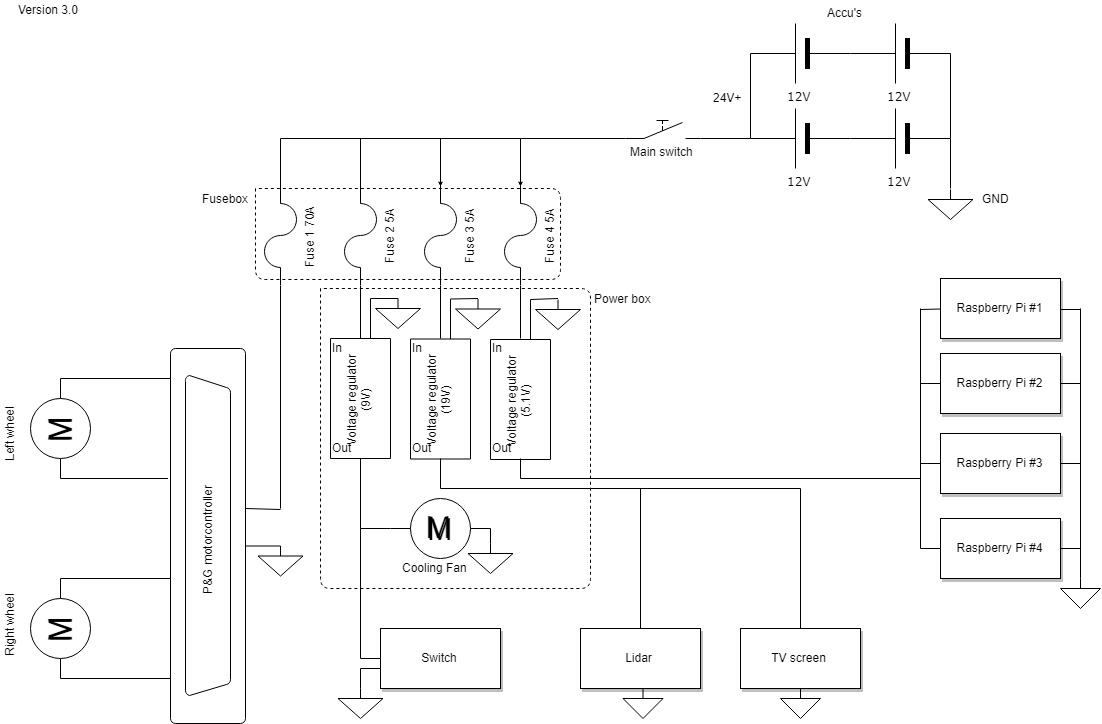
\includegraphics[width=16cm]{wiringSchem.jpg}
\caption{Schematic showing the wiring set-up of WTR}
\label{fig::wiringschem}
\end{figure}

This change was implemented because it allows a quick disengagement of the motors, rather than killing the motor controller.


\subsubsection{Fuses}
Currently, WTR uses 3 $5A$ universal car fuses, which should prevent any of the devices being overloaded.
In case this is not enough, several other fuses ranging from $5A$ to $30A$ can be found in cupboard C in the innovation lab on T5.
The electric motors are secured with a $70A$ fuse, should this not be enough a new fuse will need to be obtained, as there were no spares.

\newpage
